\chapter{Experiments}

\section{Method}

\begin{itemize}
  \item Worst case:   lowest nodes
  \item Average case: halfway in data structure
  \item Best case:    remove left side of root node
\end{itemize}

\section{Results}

\subsection{Execution Time}

% \begin{figure}[H]
%   \centering
%   \includegraphics[width=.7\textwidth]{plots/run-17/time/all_benchmarks.pdf}  
%   \caption{Results execution time for a single computation.}
%   \label{fig-bench-execution-time}
% \end{figure}

\subsection{Memory Usage}

% \begin{figure}[H]
%   \centering
%   \includegraphics[width=.7\textwidth]{plots/run-17/memory/all_benchmarks.pdf}
%   \caption{Results memory usage for a single computation.}
%   \label{fig-bench-memory-usage}
% \end{figure}

\subsection{Comparison Memory Strategies}